\tikzset{every picture/.style={line width=0.75pt}} %set default line width to 0.75pt        

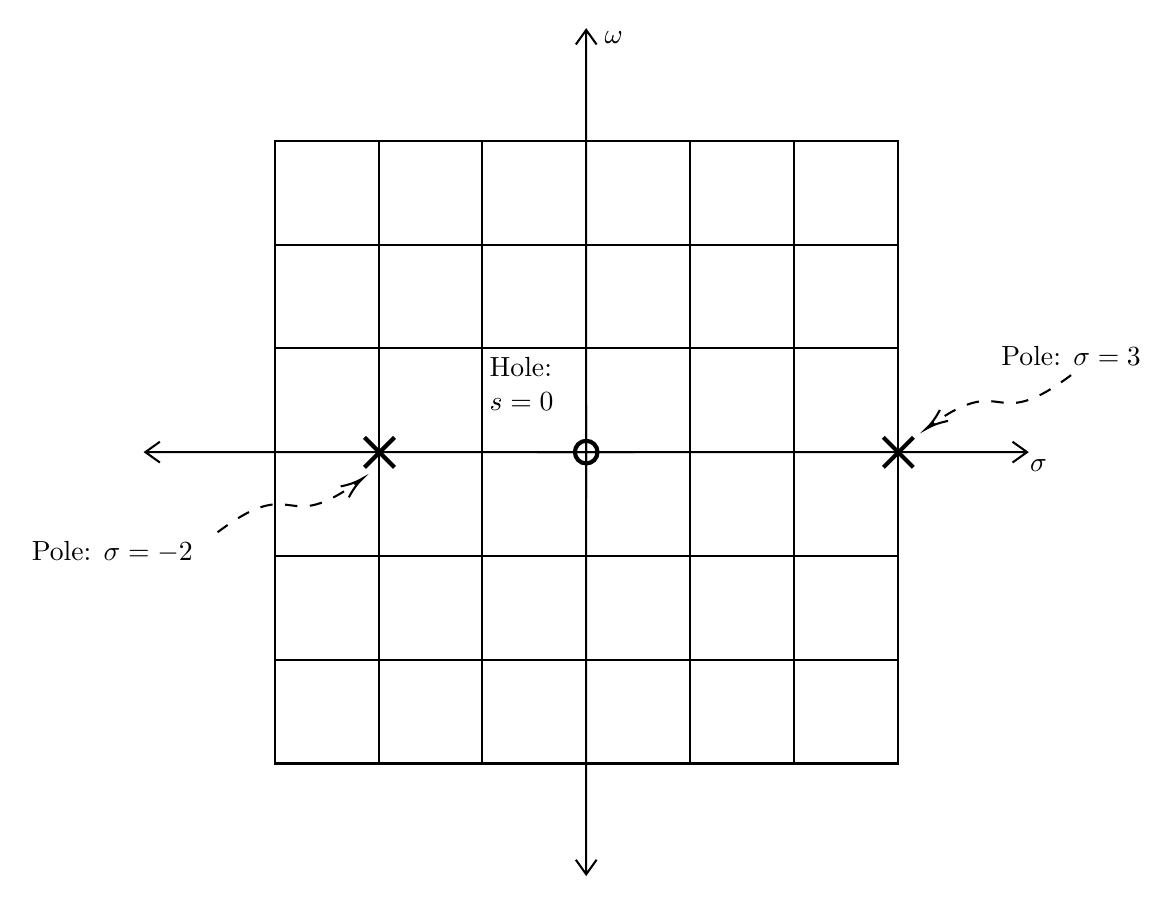
\begin{tikzpicture}[x=0.75pt,y=0.75pt,yscale=-1,xscale=1]
%uncomment if require: \path (0,413); %set diagram left start at 0, and has height of 413

%Shape: Axis 2D [id:dp07291137441905748] 
\draw  (271,207.4) -- (507,207.4)(294.6,4) -- (294.6,230) (500,202.4) -- (507,207.4) -- (500,212.4) (289.6,11) -- (294.6,4) -- (299.6,11)  ;
%Shape: Axis 2D [id:dp6518246903591405] 
\draw  (318.2,207.4) -- (82.2,207.4)(294.6,410.8) -- (294.6,184.8) (89.2,212.4) -- (82.2,207.4) -- (89.2,202.4) (299.6,403.8) -- (294.6,410.8) -- (289.6,403.8)  ;
%Shape: Grid [id:dp49490922295513473] 
\draw  [draw opacity=0] (294.6,57.4) -- (444.6,57.4) -- (444.6,207.4) -- (294.6,207.4) -- cycle ; \draw   (344.6,57.4) -- (344.6,207.4)(394.6,57.4) -- (394.6,207.4) ; \draw   (294.6,107.4) -- (444.6,107.4)(294.6,157.4) -- (444.6,157.4) ; \draw   (294.6,57.4) -- (444.6,57.4) -- (444.6,207.4) -- (294.6,207.4) -- cycle ;
%Shape: Grid [id:dp22016715431592204] 
\draw  [draw opacity=0] (294.6,207.4) -- (444.6,207.4) -- (444.6,357.4) -- (294.6,357.4) -- cycle ; \draw   (344.6,207.4) -- (344.6,357.4)(394.6,207.4) -- (394.6,357.4) ; \draw   (294.6,257.4) -- (444.6,257.4)(294.6,307.4) -- (444.6,307.4) ; \draw   (294.6,207.4) -- (444.6,207.4) -- (444.6,357.4) -- (294.6,357.4) -- cycle ;
%Shape: Grid [id:dp9168332724400642] 
\draw  [draw opacity=0] (144.6,207.4) -- (294.6,207.4) -- (294.6,357.4) -- (144.6,357.4) -- cycle ; \draw   (194.6,207.4) -- (194.6,357.4)(244.6,207.4) -- (244.6,357.4) ; \draw   (144.6,257.4) -- (294.6,257.4)(144.6,307.4) -- (294.6,307.4) ; \draw   (144.6,207.4) -- (294.6,207.4) -- (294.6,357.4) -- (144.6,357.4) -- cycle ;
%Shape: Grid [id:dp019661334699653366] 
\draw  [draw opacity=0] (144.6,57.4) -- (294.6,57.4) -- (294.6,207.4) -- (144.6,207.4) -- cycle ; \draw   (194.6,57.4) -- (194.6,207.4)(244.6,57.4) -- (244.6,207.4) ; \draw   (144.6,107.4) -- (294.6,107.4)(144.6,157.4) -- (294.6,157.4) ; \draw   (144.6,57.4) -- (294.6,57.4) -- (294.6,207.4) -- (144.6,207.4) -- cycle ;
%Shape: Circle [id:dp8466727816697135] 
\draw  [line width=1.5]  (289.15,207.4) .. controls (289.15,204.39) and (291.59,201.95) .. (294.6,201.95) .. controls (297.61,201.95) and (300.05,204.39) .. (300.05,207.4) .. controls (300.05,210.41) and (297.61,212.85) .. (294.6,212.85) .. controls (291.59,212.85) and (289.15,210.41) .. (289.15,207.4) -- cycle ;
%Straight Lines [id:da019164220491805106] 
\draw [line width=1.5]    (202.22,200.28) -- (187.78,214.72) ;
%Straight Lines [id:da7010872252517704] 
\draw [line width=1.5]    (202.22,214.72) -- (187.78,200.28) ;

%Straight Lines [id:da8787997404879367] 
\draw [line width=1.5]    (452.22,200.28) -- (437.78,214.72) ;
%Straight Lines [id:da40962171693247995] 
\draw [line width=1.5]    (452.22,214.72) -- (437.78,200.28) ;

%Curve Lines [id:da12390900966481411] 
\draw  [dash pattern={on 4.5pt off 4.5pt}]  (117,246) .. controls (156.6,216.3) and (147.2,249.33) .. (185.81,220.88) ;
\draw [shift={(187,220)}, rotate = 143.13] [color={rgb, 255:red, 0; green, 0; blue, 0 }  ][line width=0.75]    (10.93,-3.29) .. controls (6.95,-1.4) and (3.31,-0.3) .. (0,0) .. controls (3.31,0.3) and (6.95,1.4) .. (10.93,3.29)   ;
%Curve Lines [id:da10550563739707763] 
\draw  [dash pattern={on 4.5pt off 4.5pt}]  (528.22,170.28) .. controls (488.62,199.98) and (498.03,166.95) .. (459.41,195.4) ;
\draw [shift={(458.22,196.28)}, rotate = 323.13] [color={rgb, 255:red, 0; green, 0; blue, 0 }  ][line width=0.75]    (10.93,-3.29) .. controls (6.95,-1.4) and (3.31,-0.3) .. (0,0) .. controls (3.31,0.3) and (6.95,1.4) .. (10.93,3.29)   ;

% Text Node
\draw (302,3.4) node [anchor=north west][inner sep=0.75pt]    {$\omega $};
% Text Node
\draw (507,209.4) node [anchor=north west][inner sep=0.75pt]    {$\sigma $};
% Text Node
\draw (26,249) node [anchor=north west][inner sep=0.75pt]   [align=left] {Pole: $\displaystyle \sigma =-2$};
% Text Node
\draw (528.22,167.28) node [anchor=south] [inner sep=0.75pt]   [align=left] {Pole: $\displaystyle \sigma =3$};
% Text Node
\draw (246.6,160.4) node [anchor=north west][inner sep=0.75pt]   [align=left] {Hole:\\$\displaystyle s=0$};


\end{tikzpicture}
